\chapter{From T1 images to numerical simulation}
\label{chp:chp3}

The goal of this chapter is to enable numerical simulation over a
brain region defined from structural MR images. To address this
challenge, we first demonstrate how to generate a high quality mesh of
a brain hemisphere from T1-weighted MR images using the tools
introduced in Chapter~\ref{chp:chp2}. Next, we show how to define a
finite element discretization of the diffusion
equation~\eqref{eq:diffusion} over this mesh to simulate the influx of
an injected tracer.

\section{Generating a volume mesh from T1-weighted MRI}
\label{sec:chp3:tools}

To generate a mesh from an MRI data set including T1-weighted images,
we follow three main steps:
\begin{enumerate}
\item
  extract a T1-weighted image series from the MRI dataset;
\item
  create (boundary) surfaces from the T1-weighted images using FreeSurfer;
\item
  generate a volume mesh of the interior using FreeSurfer along with \svmtk.
\end{enumerate}
We will consider each of these steps in order, and encourage the
reader to ensure that FreeSurfer is installed and configured (see
Chapter~\ref{sec:chp2:tools:freesurfer}) before proceeding. Step 2 can
be particularly time consuming, likely with FreeSurfer segmentation
and reconstruction run times of up to 24 hours.
While we provide already processed files in the tarball that accompanies
the book, we encourage the reader to try it out. 
 
\subsection{Extracting a single series from an MRI dataset}

To extract a single MR series from an MRI dataset or a DICOM database,
we can use the DicomBrowser graphical interface or FreeSurfer command
line tools. The first option, using the DicomBrowser graphical
interface to extract a T1-weighted image series, was described in
Chapter~\ref{sec:chp2:viewmri} with the book data set as an example,
and the resulting image series can be found under \ernieT1 in
the book data set. The second option is described in
Chapter~\ref{sec:chp3:advanced} at the end of this chapter.

\subsection{Creating surfaces from T1-weighted MRI}
\label{sec:chp3:surfaces}

The next step is to create surfaces, representing e.g.~the interface
between the pia membrane and the surrounding CSF, here referred to as
the pial surface, or the interface between white and gray matter, from
the T1-weighted MRI series just extracted. We will use FreeSurfer for
this task, and as an example, we will extract the pial surface
surrounding the left hemisphere of a brain.

To conduct a full image stack segmentation and surface reconstruction,
we take advantage of the FreeSurfer command \emp{recon-all}. This
command is compute-intensive, with run times likely of up to 24
hours. To invoke \emp{recon-all}, we select one of the T1 DICOM files:
for instance, in~\emp{\ernieT1}, we can pick \emp{IM\_0162}. Next, we
decide on a subject identifier for the FreeSurfer pipeline; we choose
to name this example subject "ernie". We are now ready to launch
\emp{recon-all}\footnote{This is a good thing to do on a separate
  core or overnight.}:

\terminal{\$ cd \emp{\ernieT1} \\
  \$ recon-all -subjid ernie -i IM\_0162 -all}

The results of \emp{recon-all} will be output to the folder
\emp{SUBJECTS\_DIR/ernie}, where the environment variable
\emp{SUBJECTS\_DIR} defaults to the \emp{subjects} folder under
\emp{FREESURFER\_HOME} (see
Chapter~\ref{sec:chp2:tools:freesurfer}). For convenience, this output
is also included in the book data set, under \emp{\ernieoutput}. If we
inspect the contents of this directory we will see several
subdirectories; some important subdirectories are:
\begin{itemize}
\item \emp{/stats}: contains files providing statistics derived during segmentation.
\item \emp{/mri}: contains volume files generated during segmentation
\item \emp{/surf}: contains surface files generated during segmentation
\end{itemize}

To view the generated surface files, we focus on the \emp{/surf}
directory, and launch freeview (see
Chapter~\ref{sec:chp2:tools:freesurfer}):
\terminal{\$ cd \ernieoutput/surf\\
\$ freeview \&}
\noindent Targeting the pial surface that surrounds the left brain
hemisphere as an example, select \button{File$\rightarrow$Load Surface}
from the command bar, and then select the file titled \emp{lh.pial}
(\emp{lh} refers to left hemisphere and \emp{pial} denotes the pial
surface). After a moment the view windows will be populated with 2D
surface slices shown as curves, in addition to a reconstructed 3D
image of the pial surface (Figure~\ref{fig:chp3:freeview-scr}).
\begin{figure}%\sidecaption
  \centering
  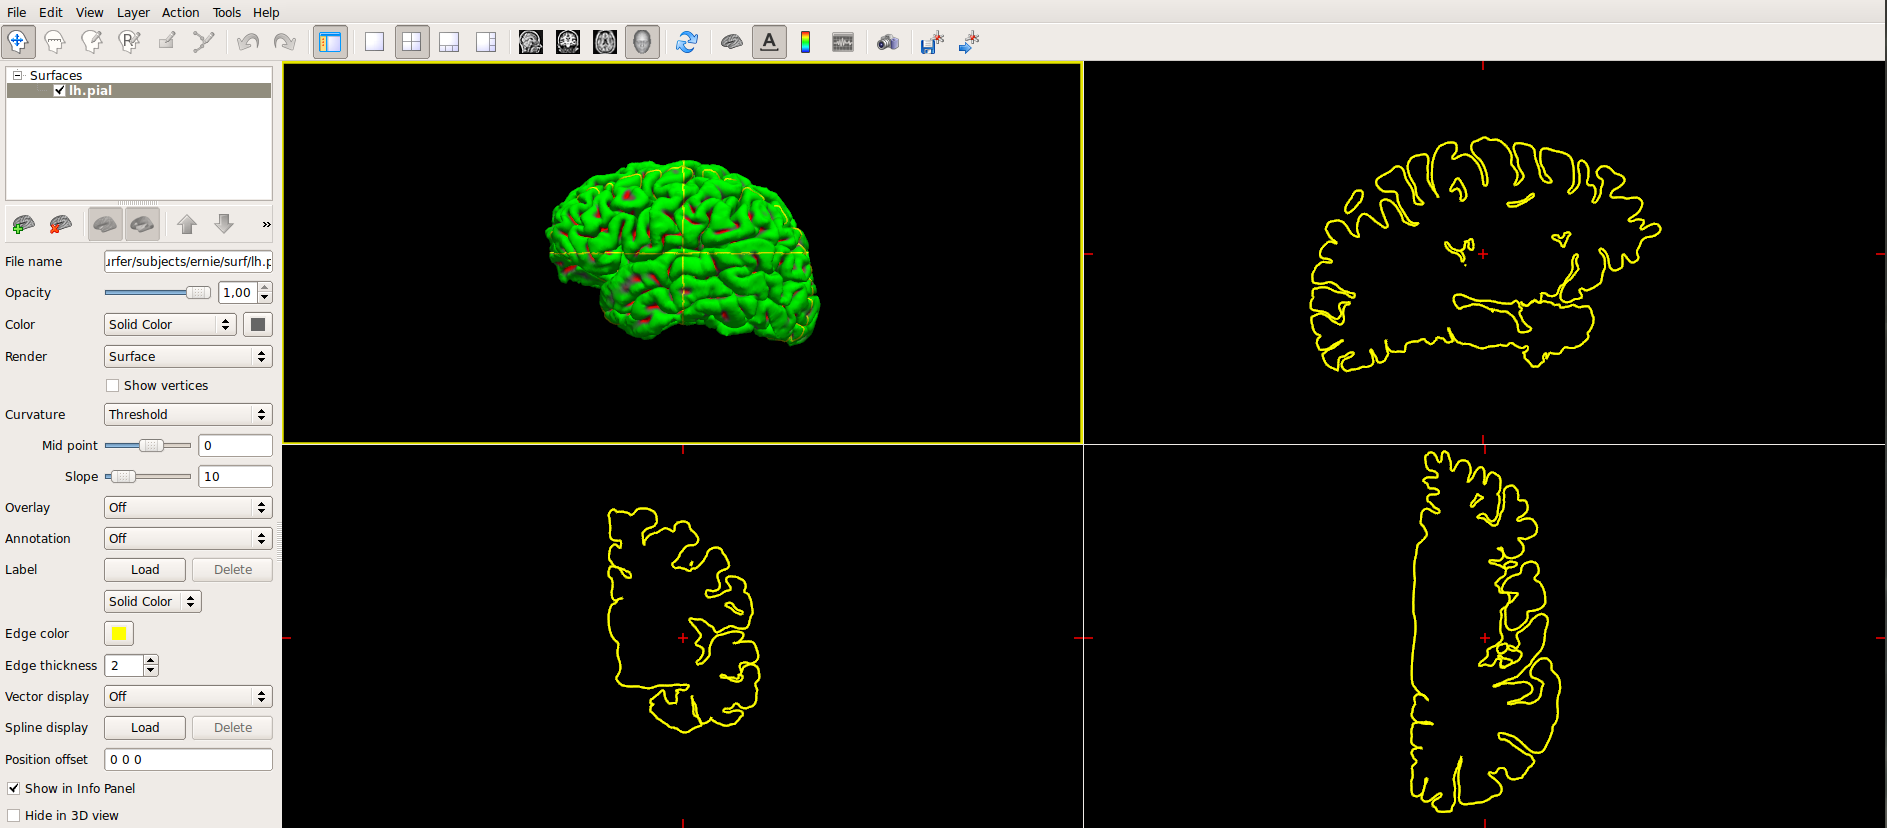
\includegraphics[width=0.95\textwidth]{./chapters/chp3/FIG/freeviewexscr}
  \caption{Freeview visualization of the pial surface of a single
    brain hemisphere extracted from T1 images via FreeSurfer.}
  \label{fig:chp3:freeview-scr}
\end{figure}

To work further with this surface, we use the FreeSurfer tool
\emp{mris\_convert} to convert it into the STL
format~\cite{roscoe1988stereolithography}. STL is a widely used format
representing the surface discretely in terms of vertices, triangles
and normals. In general, \emp{mris\_convert} is used to handle the
conversion between different surface formats. For instance, in the
directory \emp{\ernieoutput/surf}, we can run

\terminal{\$ mris\_convert ./lh.pial pial.stl}

\noindent to create the file \emp{lh.pial.stl} in the current
directory. The resulting file can be opened in several different
programs, for instance in ParaView or Gmsh.

\subsection{Creating a volume mesh from a surface}
\label{subsec:chp3:mesh-creation}

The third step of our initial meshing pipeline is to generate a mesh
of the volume bounded by the surface representation. We will use the
tailored package \svmtk{} (see
Chapter~\ref{sec:chp2:tools:meshing:svmtk}) to convert from the STL
surface representation to a volume mesh. The Python script below (
\emp{mri2fem/chp3/surface\_to\_mesh.py} in the book scripts)
demonstrates this fundamentals of this process. The script (and all
similar scripts in the following) can then be run from there as
\terminal{\$ python surface\_to\_mesh.py}

The script defines a Python function
\pythoninline{create\_volume\_mesh} which can be called as
\newpythonsnippet{chp3}{surface_to_mesh.py}{15}{16}

\noindent The function itself reads as
\newpythonsnippet{chp3}{surface_to_mesh.py}{0}{12}

\noindent Given an input STL filename (\pythoninline{stlfile}), an
output mesh filename with the \pythoninline{mesh} suffix
(\pythoninline{meshfile}), and an optional mesh resolution
(\pythoninline{resolution}, defaulting to 16), the script creates an
\svmtk{} \pythoninline{Domain} object, generates a mesh from the
surface via the call to \pythoninline{create\_mesh}, and saves this
mesh in the \pythoninline{.mesh} format to the output mesh file. The
mesh resolution parameter determines the maximum size of a tetrahedron
in the volume mesh (relative to the overall bounding box length for
the input surface): the higher the value, the higher the resolution,
i.e.~the smaller the area of each element in the volume mesh
generated. Figure \ref{fig:chp3:ernie-volume-mesh} shows meshes with
\pythoninline{resolution = 16} (left) and \pythoninline{resolution =
  64} (right). Mesh generation can be a costly operation, with higher
run times (of the order seconds to minutes) for higher resolutions.
\begin{figure}
  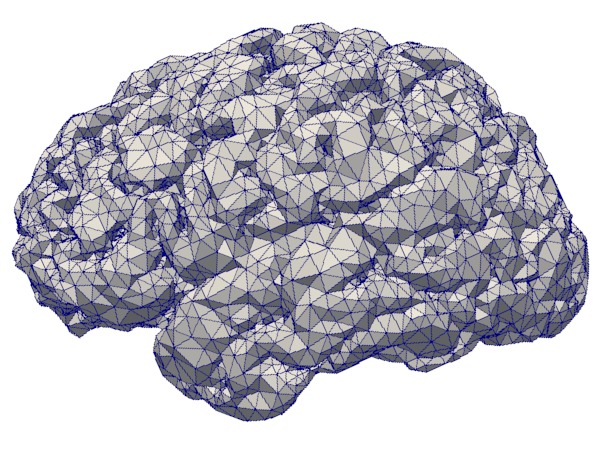
\includegraphics[width=0.49\textwidth]{./chapters/chp3/FIG/ernie-volume-16-r.png}
  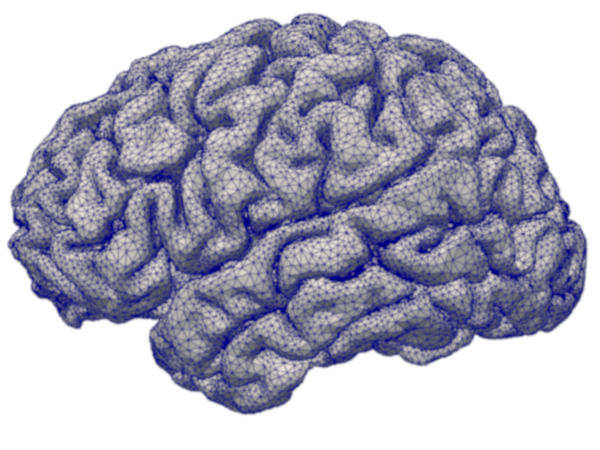
\includegraphics[width=0.49\textwidth]{./chapters/chp3/FIG/ernie-volume-64-r.png}
  \caption{Volume meshes of a left brain hemisphere produced by
    {\svmtk} from STL surface files -- with lower (left) and higher
    (right) mesh resolutions.}
  \label{fig:chp3:ernie-volume-mesh}
\end{figure}

%\kam{I don't understand the explanation for the resolution. 
%is the formula $(\mbox{bounding box}/\mbox{ tet volume})^{1/3}$ }

The \emp{.mesh} format is the standard mesh format for \svmtk{} and
CGAL. However, it is not native to \fenics{}, and therefore we need to
convert the mesh to a \fenics-supported file format (e.g.~.xml, .xdmf,
.h5). The Python package meshio (see~Chapter
\ref{sec:chp2:meshio}) is well-suited for this purpose and can
convert between many different input and output mesh formats. For
instance, to convert to the FEniCS .xdmf format, we can run
\terminal{\$ meshio-convert lh.mesh lh.xdmf}
\noindent The .xdmf file can then be viewed in e.g.~ParaView.

\section{Improved volume meshing by surface preprocessing}
\label{sec:chp3:improved-volume-meshing}
In the previous section, we stepped through the main pipeline for
generating a volume mesh from MR images. However, the brain surfaces
generated from T1 images often have a number of weaknesses:
\begin{itemize}
\item the surfaces may have unphysiologically sharp corners,   
\item the surfaces may include triangles with very large aspect ratios, 
\item the surfaces may have topological defects such as holes, and
\item the surfaces may self-intersect or overlap with other surfaces.   
\end{itemize}
These defects can cause the volume mesh generation to fail or result
in low quality meshes that are not suitable for numerical
simulation. Therefore, surface preprocessing is often required to
enhance surface quality prior to generating volumetric meshes. Here,
we outline three main aspects of surface preprocessing: remeshing,
smoothing and separation. The enhanced STL surfaces can then be
directly inserted into the volume mesh generation described above in
Chapter~\ref{subsec:chp3:mesh-creation}.

\subsection{Remeshing a surface}
\label{subsubsec:chp3:mesh-creation:remeshing}

To increase surface or volume mesh quality, we can remesh the original
surface representation. The remeshing can, for instance, reduce the
frequency of mesh cells that are overly distorted and reduce the
density of vertices with a large number of connected edges.

\svmtk{} includes utilities for remeshing surface files, and we can
remesh our original surface \emp{lh.pial.stl} e.g.~via the
following script (included as \emp{mri2fem/chp3/remesh\_surface.py} in
the book scripts). We define a short Python function
\pythoninline{remesh_surface} that can be called as
\newpythonsnippet{chp3}{remesh_surface.py}{16}{17}
\noindent The function itself reads as
\newpythonsnippet{chp3}{remesh_surface.py}{0}{15}

\noindent Here, we read the input STL file as an \svmtk{}
\pythoninline{Surface}, and remesh using
\pythoninline{isotropic\_remeshing}, before saving the remeshed
surface, again as an STL file. We can specify more iterations, and
produce a finer mesh, by increasing the integer value of
\pythoninline{n}. The floating point value of \pythoninline{L}
indicates the maximum edge length of a mesh cell. Surfaces generated
by FreeSurfer are typically in millimeters (mm), and the volume meshes
inherits this unit. The boolean
\pythoninline{do\_not\_move\_boundary\_edges} defines whether \svmtk{}
is allowed to move the boundary vertices during the remeshing
procedure (\pythoninline{False}) or not (\pythoninline{True}). It is
generally advised to allow boundary vertices to move, as requiring
these to be fixed can cause the remeshing to fail.

Figure \ref{fig:chp3:ernie-remesh} shows the result
\emp{lh.pial.remesh.stl} with three remeshing iterations on the raw
input file \emp{lh.pial.stl}; the figure has been zoomed in to draw
attention to local feature differences. Both files have been viewed
and visualized in ParaView.
\begin{figure}
  \centering
  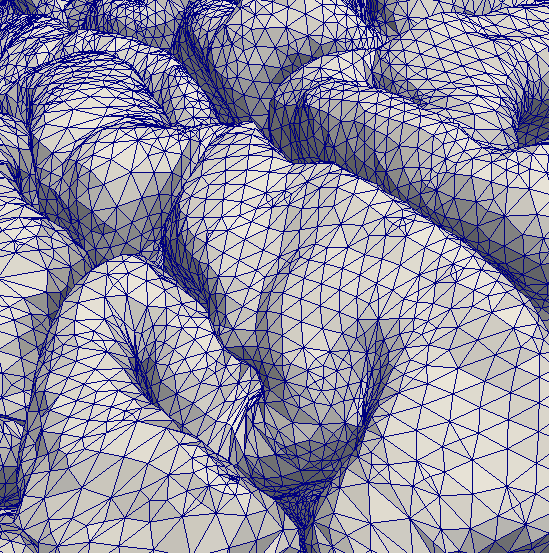
\includegraphics[width=0.49\textwidth]{./chapters/chp3/FIG/raw-stlmesh.png}
  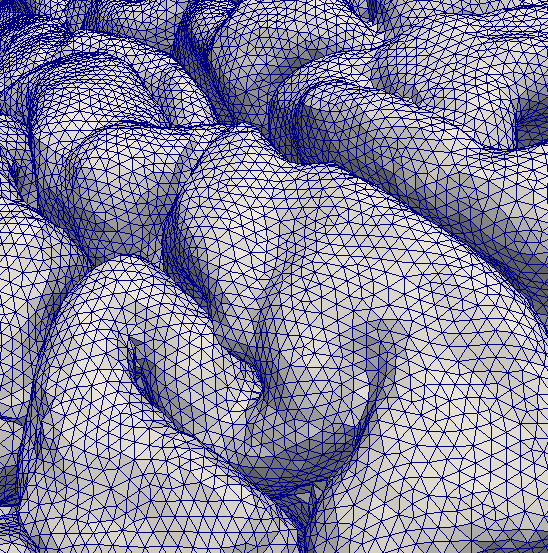
\includegraphics[width=0.49\textwidth]{./chapters/chp3/FIG/remesh-stlmesh.png}
  \caption{Original (left) pial surface and (right) after remeshing with \svmtk{}}
  \label{fig:chp3:ernie-remesh}
\end{figure}


\subsection{Smoothing a surface file}
\label{subsubsec:chp3:mesh-creation:smoothing}

To reduce the presence of non-physiological features such as sharp
corners, it may be advantageous to smoothen the surfaces prior to
meshing. \svmtk{} also includes utilities for smoothing surfaces, as
we demonstrate in the below script (included as
\emp{mri2fem/chp3/smooth\_surface.py} in the book scripts) -- using
our remeshed surface \emp{lh.pial.remesh.stl} as sample input.

Again, we define a short Python function
\pythoninline{smoothen\_surface} that can be called as
\newpythonsnippet{chp3}{smooth_surface.py}{19}{20}
\noindent The function itself reads as
\newpythonsnippet{chp3}{smooth_surface.py}{0}{17}

The boolean variable \pythoninline{preserve\_volume} determines
whether a volume-preserving Taubin smoothing (\pythoninline{True}) or
not-necessarily volume preserving Laplacian smoothing
(\pythoninline{False}) process should be used.  From a conceptual
point of view, a Taubin smoothing is essentially a local smoothing
iteration followed by a local "swelling" operation which preserves the
volume of the original patch, whereas the Laplacian smoothing consists
only of local smoothing operations and the volume of the original
patch may not be preserved \cite{taubin1995curve}. Of the two, we
recommend using Taubin smoothing. The integer value \pythoninline{n}
sets the number of times the smoothing process should occur. Higher
values will produce a smoother mesh; however, too high of a value may
result in a loss of resolution in brain features such as the sulci and
gyri (grooves and bumps) on the brain surface. Finally, the floating
point value \pythoninline{eps} determines the strength of the
smoothing operation for each smoothing iteration, and should be in the
interval $[0, 1]$ with $0.0$ (resp.~$1.0$) indicating no (resp.~full)
smoothing.
\begin{figure}
  \centering
  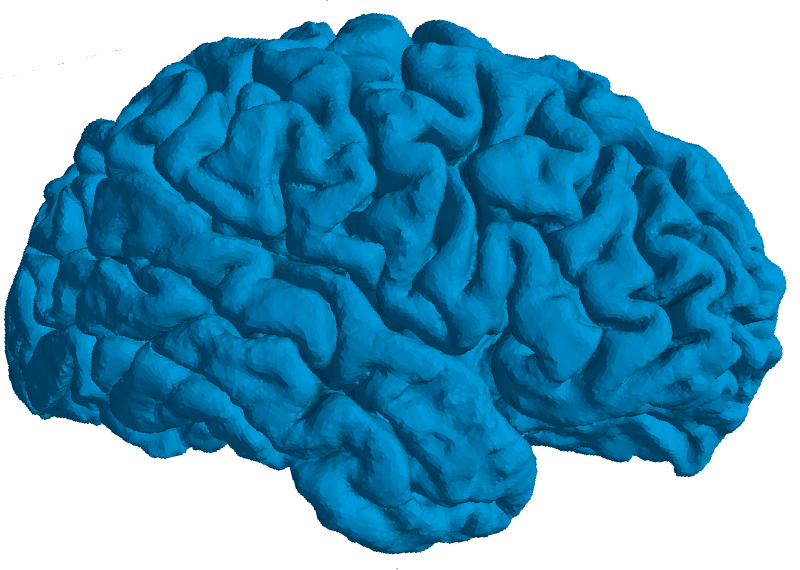
\includegraphics[width=0.30\textwidth]{./chapters/chp3/FIG/unsmoothed.png}
  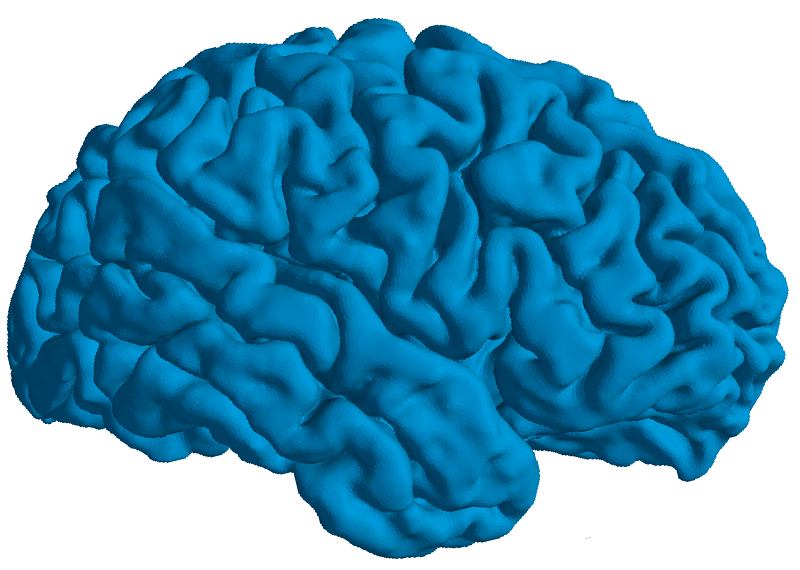
\includegraphics[width=0.30\textwidth]{./chapters/chp3/FIG/taubin-smoothed-10.png}
  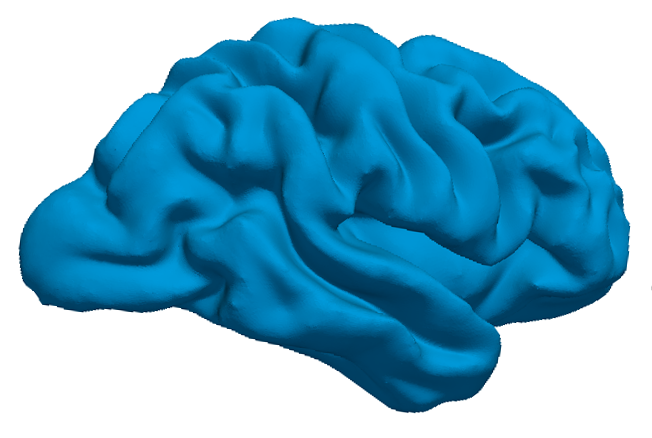
\includegraphics[width=0.30\textwidth]{./chapters/chp3/FIG/oversmoothing.png}
  \caption{Surface smoothing: original pial surface 
    (\emp{lh.pial.remesh.stl}, left) and after Taubin smoothing with
    {\svmtk} (\emp{lh.pial.smooth.stl}, middle), and Laplacian over-smoothing (right).}
  \label{fig:chp3:ernie-smoothing}
\end{figure}
Figure~\ref{fig:chp3:ernie-smoothing} shows the result of ten
iterations of Taubin smoothing. On the other hand, over-smoothing of
the pial surface can lead to missing anatomical detail or errors, see
e.g.~Figure~\ref{fig:chp3:ernie-smoothing}. It is generally advised to
check the file visually by opening it directly, using either ParaView
or Gmsh, to determine if more or less smoothing is needed; some
surface STL files may require more, or fewer, iterations than others.

We can generate a higher quality mesh in XML or XDMF format by
generating the volume mesh from the remeshed and smoothened STL
surface using the Python call
\begin{python}
create_volume_mesh("lh.pial.smooth.stl", "ernie.mesh")
\end{python}
followed by
\terminal{\$ meshio-convert ernie.mesh ernie.xml\\
\$ meshio-convert ernie.xml ernie.xdmf}
\noindent We will use the resulting \emp{ernie.xdmf} in the
simulations ahead in Chapter~\ref{sec:chp3:math}.

\subsection{Preventing surface intersections and missing facets}
\label{subsec:chp3:preventing-surface-intersections}

%In FreeSurfer, the right and left hemisphere surfaces are generated
%separately. Combining surfaces from different hemisphere can create
%problems such as:
%\begin{itemize}
%\item the hemisphere surfaces overlap, creating bridges in the cortical gray matter;
%\item the hemisphere surfaces do not overlap, creating gaps in the white matter. 
%\end{itemize} 
%We can consider this a combined problem, since we typically would want
%to join the hemisphere surface via the white matter nerve tracts, but
%avoid overlapping surfaces in the cortical gray matter. \svmtk{} also
%includes utilities for such operations:
%\item
%  \pythoninline{separate\_overlapping\_surfaces}: for iteratively
%  separating overlapping surfaces;
%\item
%  \pythoninline{separate\_close\_surfaces} for iteratively separating
%  nearly overlapping surfaces. (We can also add a third surface to the
%  function, such as the union of the white surfaces, to avoid moving
%  the vertices that are inside this third surface.);

\svmtk{} also includes utilities for repairing surface faults:
\begin{itemize}
\item
  Surfaces constructed by FreeSurfer can have topological defects,
  such as holes, these defects can be repaired by following the
  FreeSufer Topological defects tutorial guide~\cite{freesurfer-wiki}.
  But, we can also encounter surfaces that have missing facets,
  i.e. structural defects, which can be corrected with the \svmtk{}
  function \pythoninline{fill\_holes}.
\item
  The foldings of pial surfaces can produce narrow gaps. Gaps that are
  shorter than the edge size of the mesh may result in bridges instead
  of foldings in the mesh, as exemplified in
  Figure~\ref{fig:chp3:juncture}. The function
  \pythoninline{separate\_narrow\_gaps} % can iteratively separate
  close junctures until the edge distance between vertices is less
  than the distance between unconnected vertices. The iterative
  separation is performed by multiplying the outward surface normal
  with a user-specified negative value. 
\item 
  The command \pythoninline{collapse\_edges} will combine short edges
  such that the new edge lengths equals to the input target edge
  length.
\end{itemize}
\begin{figure}\sidecaption
  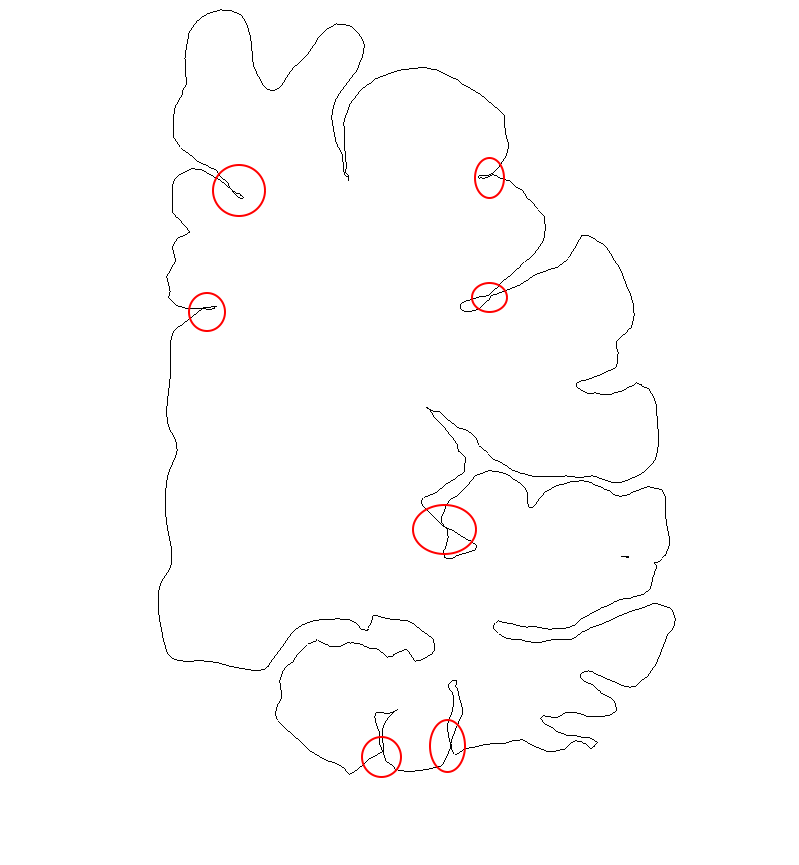
\includegraphics[width=0.5\textwidth]{./chapters/chp3/FIG/juncturers-gap.png}
  \caption{Illustration of close junctures in a coronal
    slice of the pial surface created by FreeSurfer.}
  \label{fig:chp3:juncture}
\end{figure}
The following Python snippet illustrates the use of these commands
(included as \emp{mri2fem/chp3/svmtk\_repair\_utilities.py} in the
book scripts). More commands involving multiple surfaces will be
covered in Chapter \ref{chp:chp4}.
\newpythonsnippet{chp3}{svmtk_repair_utilities.py}{0}{11}

\section{Simulation of diffusion into the brain hemisphere}
\label{sec:chp3:math}

With a mesh representing the domain of interest, we are ready to start
modelling and numerically simulating biophysical processes in this
domain. As a first example, we will study diffusion into the brain
parenchyma of a tracer injected in the subarachnoid space. This is a
setting encountered e.g.~in clinical practice when gadobutrol are
injected intrathecally (into the cerebrospinal fluid in the spinal
cord subarachnoid space)~\cite{ringstad2018brain}, and in experimental
research when fluorescent tracers such as dextran are injected in the
cisterna magna of mice~\cite{iliff2012paravascular,
  xie2013sleep}. Understanding the role of diffusion -- versus other
mechanisms such as convection -- in the brain parenchyma is a topic of
substantial interest in physiology and medicine~\cite{abbott2018role}.

%% A recent clinical experiment \cite{ringstand-2018-journal} has aimed
%% to test the communication of the subarachnoid CSF compartment and the
%% extravascular component of human brain tissue; such communication is
%% postulated by the glymphatic hypothesis.  The study was conducted
%% using MRI imaging alongside the injection of a tracer into the
%% subarachnoid CSF.  Following injection, the clinicians then observe
%% how the tracer makes its way through the brain and examine the
%% time-to-clearance of this tracer for both reference patients and a
%% cohort with dementia.

\subsection{Research question and model formulation}
\label{chp3:model}

Let us ask the following question: assuming that solutes move in the
brain parenchyma by diffusion alone, given an intrathecal injection of
the contrast agent gadobutrol as in glymphatic MRI
investigations~\cite{ringstad2018brain}, what would be the evolution
and distribution patterns of gadobutrol in the brain -- up to 24 hours
after injection?

To begin addressing this question, we define an initial-boundary-value
problem for the diffusion of gadobutrol in the brain parenchyma. To do
so, we need to prescribe the computational domain, initial conditions,
parameter values, and boundary conditions for \eqref{eq:diffusion}. It
is often a good idea to also think about the units when defining your
simulation scenario. In brain mechanics at the tissue or organ level,
millimeters (mm) or meters (m) and seconds (s) or minutes (min) are
often suitable choices of units -- noting of course that some
physiological processes happen on the order of days, months or years.

Here, we let the concentration $u$ represent the (unit-less)
concentration of gadobutrol solving~\eqref{eq:diffusion} in
$\Omega$. The image-based mesh of the left brain hemisphere
(e.g.~\emp{ernie.xdmf}) defines the computational domain
$\Omega$. Formally, $\Omega$ is then the union of the cells in the
mesh. Note that the mesh defines the spatial coordinates of the domain
- and as a consequence the spatial unit. Meshes generated from
FreeSurfer data are typically defined in terms of mm, and thus mm is
the default unit for the spatial scale. The spatial unit can be
redefined by rescaling the mesh -- this is a simple operation in
FEniCS. We also pick a final time and time unit, for instance $T =
1440$ min ($T = 24$ hours).

We assume that there is no gadobutrol present in the domain initially,
which translates to the initial condition:
\begin{equation}
  \label{eq:chp3:ic}
  u_0(x, 0) = 0 \quad \text{ for all } x \in \Omega.
\end{equation}
Next, we assume that gadobutrol is distributed to the brain surface
via the cerebrospinal fluid in the subarachnoid space by setting the
boundary condition:
\begin{equation}
  \label{eq:chp3:bc}
  u_d(x, t) = 2.813 \times 10^{-3} \quad x \in \partial \Omega, \quad t > 0
\end{equation}
%% \kam{some details concerning why the specific value
%% $2.813 \times 10^{-3}$ 
%% is choosen?
%% I also do not understand the above discussion of $\Omega$ and $\mesh$.  
%% Is $\Omega$ the union of cells in $\mesh$ is it the real domain which 
%% we approximate? 
%% }
where $\partial \Omega$ denotes the boundary of $\Omega$, which
represents the pial surface in this scenario. Assuming that the
concentration is known on the pial surface everywhere and at all times
is clearly a simplification. More realistic boundary conditions can
and have been considered in the literature~\cite{valnes2020apparent,
  croci2019uncertainty}, and one could also directly model the
movement of tracer in the cerebrospinal fluid in the subarachnoid
space~\cite{haga2017numerical,pizzichelli2017numerical}

Brain tissue is heterogeneous and anisotropic -- which means that the
effective diffusion tensor $K$ in~\eqref{eq:diffusion} should vary in
space (and probably in time over longer time scales) and be
tensor-valued. We will address these aspects later in this book (in
Chapter~\ref{chap:dti}), but for now we just consider a uniform and
single-valued $K$. We estimate the
average effective diffusion coefficient of gadobutrol in brain tissue
to be
\begin{equation}
  K  
  = 4.32 \times 10^{-1} \, \text{mm$^2$/hour}
  = 7.2 \times 10^{-3} \, \text{mm$^2$/min}
\end{equation}
Finally, we assume that there are no sources or sinks of gadobutrol
within the brain parenchyma and thus set
\begin{equation}
  f(x, t) = 0 \quad x \in \Omega, \quad t > 0.
\end{equation}
Again, this is clearly a simplification that does not account for
potential exit pathways for gadobutrol from the parenchyma.

%\kam{Is the above based on values from some of our studies? I think
%that would be cool. Is it UQ by Croci/Vinje/Rognes? }

\subsubsection{Quantities of interest}
The computed solution $u$ will vary in time and space and thus encodes
a substantial amount of information. We are often interested in first
merely inspecting the solution visually or qualitatively. For more
quantitative analysis and comparison with experimental or clinical
findings, we typically compute quantities of interest associated with
the solution. These quantities of interest can for instance be the
total volume of solute in the entire domain over time:
\begin{equation}
  \label{eq:chp3:qoi}
  Q(t) = \int_{\Omega} u (t) \dx, 
\end{equation}
the average concentration in local regions, or the concentration in
specific points $x$ over time: $u(x, t)$.

\subsection{Numerical solution of the diffusion equation}
\label{sec:chp3:model-problem-numerical-formulation}

To compute numerical solutions of the diffusion
equation~\eqref{eq:diffusion} in general, and our specific
initial-boundary-value problem in particular, we will use a finite
difference discretization in time and a finite element discretization
in space~\cite{langtangen2019introduction,
  gockenbach2006understanding}. This is a common approach, and we will
implement this numerical scheme using the FEniCS Project
software~\cite{logg2012automated,alnaes2015fenics,langtangen2016solving}. As
mentioned in our introductory remarks, we strongly encourage readers
unfamiliar with numerically solving PDEs or FEniCS to study the FEniCS
tutorial~\cite{langtangen2016solving} before proceeding.

For the discretization in time, we define a set of discrete times $0 =
t_0 \leq t_1 \dots \leq t_N = T$, where $N$ is the number of time
steps and the time step (size) $\tau_n = t_n - t_{n-1}$ for $n = 1,
\dots, N$. Our aim is to compute approximate solutions $u^n_h$
of~\eqref{eq:diffusion} such that $u^n_h \approx u(t^n)$ for each
$n$. To this end, we introduce the (first-order, backward) finite
difference approximation in time:
\begin{equation}
  u(t_n) \approx u^n, \quad
  u_t(t_n) \approx \frac{1}{\tau_n} (u^n - u^{n-1}),
\end{equation}
and obtain the time-discrete equations for $n = 1, \dots, N$:
\begin{equation}
  \label{eq:chp3:time-discrete}
  \frac{1}{\tau_n} (u^n - u^{n-1}) - \Div K \Grad u^n = f(t^n) \quad \text{in } \Omega. 
\end{equation}

Next, for the finite element discretization in space, we derive a
discrete variational formulation of~\eqref{eq:chp3:time-discrete} by
multiplying by test functions $\phi$ in a finite element space $V$
defined relative to the mesh $\mesh$, integrating by parts, and moving
all known terms to the right hand side, to obtain the following fully
discrete problem: find the discrete solution $u_h^n \in V$ at each
time $n = 1, \dots, N$ such that
\begin{equation}
  \label{eq:chp3:discrete}
  \inner{u_h^n}{\phi} + \tau_n \inner{\Grad u_h^n}{\Grad \phi}
  =  \inner{u_h^{n-1}}{\phi} + \tau_n \inner{f^n}{\phi},  
\end{equation}
for all test functions $\phi \in V$, and where we have used the
$L^2(\Omega)$-inner product notation
\begin{equation}
  \inner{u}{\phi} = \int_{\Omega} u \, \phi \dx.
\end{equation}
In addition, we enforce that the discrete solution should satisfy the
boundary condition~\eqref{eq:chp3:bc}, and initially be given by the
initial condition~\eqref{eq:chp3:ic}. 

The fully discrete equation~\eqref{eq:chp3:discrete} is a good
starting point for the FEniCS implementation of this scheme. We choose
to approximate the solution using continuous piecewise linear finite
element spaces. 

\subsection{Implementation using {\fenics}}
\label{sec:chp3:fenics-code-implementation}

Our model problem is very similar to the heat equation problem
presented in the FEniCS tutorial~\cite[Chapter
  3.1]{langtangen2016solving}, and we base our implementation on the
algorithm and code presented there. We begin by importing the Python
module \pythoninline{fenics}, and we also import \pythoninline{numpy}
as a handy Python module for general numerics:
\newpythonsnippet{chp3}{diffusion.py}{0}{2}

\noindent We then read the mesh that we have just generated into the FEniCS
program. We use the XDMF mesh format and reader as it is suitable for
large scale simulations and works seamlessly with MPI-parallel computing:
\newpythonsnippet{chp3}{diffusion.py}{4}{13}

\noindent We now define the parameters for the time discretization. We
choose to simulate up to 72 hours, and choose a time step $\tau$
(\pythoninline{tau}) of 3 min. Note that we use a Constant to
represent \pythoninline{time}, this is useful for updating functions
depending on time later. Also, keeping track of the parameter units
used is good practice. Here we just use the comments, while much more
rigorous solutions such as e.g.~SymPy's Unit
systems~\cite{meurer2017sympy} could be used.
\newpythonsnippet{chp3}{diffusion.py}{15}{18}

\noindent We also define the diffusion coefficient, source function
and initial condition (even though the latter two are just zero):
\newpythonsnippet{chp3}{diffusion.py}{20}{25}

We now move on to consider the specification of the finite element
discretization. We first define the finite element space $V$ as the
"Lagrange" elements of degree 1 defined relative to our mesh, and then
define a \pythoninline{TrialFunction} and \pythoninline{TestFunction}
over this space. 
\newpythonsnippet{chp3}{diffusion.py}{27}{30}

\noindent We next define a \pythoninline{Function} to hold the value
of the solution at the previous time step \pythoninline{u_}, and
initialize this function with the initial condition \pythoninline{u0}:
\newpythonsnippet{chp3}{diffusion.py}{32}{35}

\noindent Having defined these objects, we can express the variational
problem~\eqref{eq:chp3:discrete}, to be solved at each time step, in
code. We also redefine \pythoninline{u} as a
\pythoninline{Function} to represent the solution at the current time:
\newpythonsnippet{chp3}{diffusion.py}{37}{42}

\noindent Having defined the finite element space, we can also define
the boundary condition -- this will be imposed on the linear system of
equations at each time step. Note how we let the boundary value
\pythoninline{u_d} depend on the previously defined
\pythoninline{Constant} \pythoninline{time}. This way, when
\pythoninline{time} updates, so will \pythoninline{u_d} and
\pythoninline{bc}.
\newpythonsnippet{chp3}{diffusion.py}{44}{48}

We have now defined all the elements of the model problem and
numerical method and can start stepping through the solution
algorithm. Since the bilinear form on the left hand side
of~\eqref{eq:chp3:discrete} does not vary in time, we can assemble
this matrix once, outside the time loop, for the sake of efficiency:  
\newpythonsnippet{chp3}{diffusion.py}{50}{52}

We define a PVD file (indicated by suffix \pythoninline{.pvd}) for
storing the computed solution at each time step in VTK format, and
store the initial solution. This is a file format convenient for
visualization in ParaView. Note that it is not a convenient format for
reading the functions back into FEniCS however; for this purpose one
should instead use the XDMF or h5 formats.
\newpythonsnippet{chp3}{diffusion.py}{54}{57} We compute
the number of time steps \pythoninline{N} and initialize numpy arrays
for storing computational quantities of interest at each time step,
such as the total amount of solute (\pythoninline{amounts})
cf.~\eqref{eq:chp3:qoi}, and the concentration (\pythoninline{concs})
in a specific point (\pythoninline{p}).
\newpythonsnippet{chp3}{diffusion.py}{59}{65}

Now, we are ready to start stepping through time and solve the finite
element system at each time step. We first increment
\pythoninline{time} with the timestep\pythoninline{tau}, we assemble
the right hand side into the vector \pythoninline{b}, apply the
Dirichlet boundary condition, solve the resulting linear system using
an iterative solver ("gmres", "amg"), and update the previous solution
with the current solution.
\newpythonsnippet{chp3}{diffusion.py}{67}{82} We can
compute the total amount of solute by integrating the concentration
over the domain, and the concentration in the specified point by
evaluating the computed solution in this point. We also store the
entire solution to the PVD file. Writing the solution to file can take
some time, and, for fine time steps, it may often be practical to only
do this say every 2nd, or 10th or 100th time step.
\newpythonsnippet{chp3}{diffusion.py}{84}{93}
It can also be practical to store the computed quantities to file
(and rather reread for plotting):
\newpythonsnippet{chp3}{diffusion.py}{95}{98}

\index{matplotlib}
The Python module matplotlib offers quick and convenient plotting, and
we use this module to plot the quantities of interest (the total
amount of solute, and the concentration in the given point) over time,
and save these in for instance PNG format. The resulting plots are
shown in Figure~\ref{fig:chp3:png-plots}. The complete script
(including the plot code) is available in the book scripts
(\emp{mri2fem/chp3/diffusion.py}).
\begin{figure}
    \begin{tabular}{cc}
    \imagetop{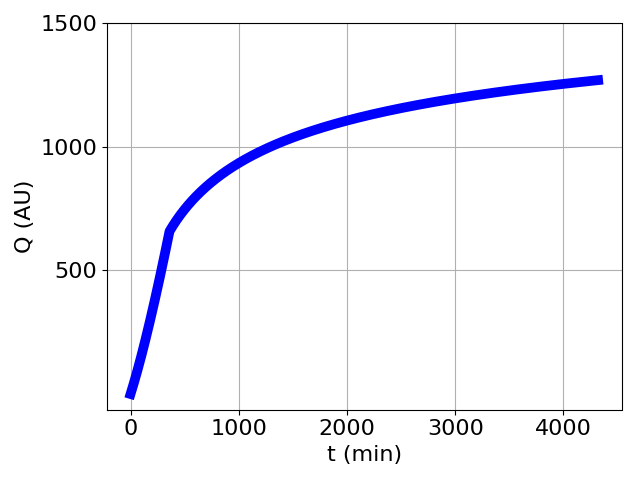
\includegraphics[width=0.49\textwidth]{./chapters/chp3/FIG/amounts.png}} &
    \imagetop{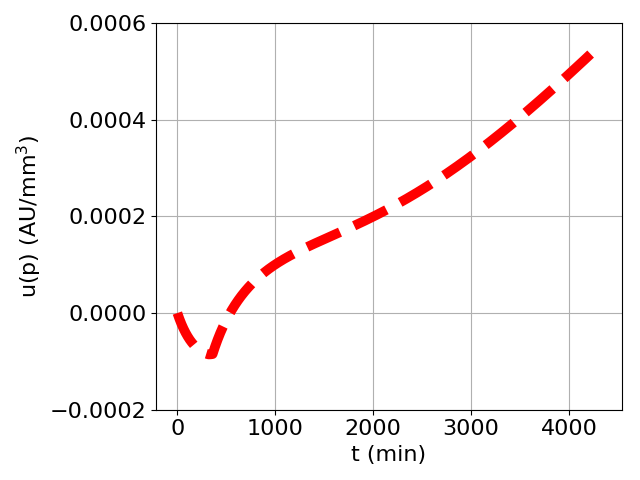
\includegraphics[width=0.49\textwidth]{./chapters/chp3/FIG/concentrations.png}}
    \end{tabular}
    \caption{Plots of quantities of interest associated with the
      computed concentration solution: total amount of solute $Q$ over
      time $t$ (left) and concentration of solution $u(p, t)$ for a
      given point $p$ over time $t$ (right).}
    \label{fig:chp3:png-plots}
\end{figure}

\index{mass lumping}
The approximation of the solute concentration at a given point over
time demonstrates an interesting numerical artifact: the concentration
drops below zero to become negative at early times (between 0 and 550
min). Negative solute concentrations are clearly unphysiological, but
a common numerical problem with diffusion simulations. A partial and
often used remedy, including in the context of diffusion simulations
in the brain~\cite{croci2019uncertainty}, is \emph{mass lumping}. Mass
lumping can reduce spurious negative concentrations, but may worsen
the overall convergence of the numerical solutions, and we will return
this aspect in Chapter~\ref{chp:chp6}.

\subsection{Visualization of solution fields}
To visualize computed solution fields, for instance, the
concentrations stored in u.pvd (and the associated u*.vtu files) in
the previous section, we will use ParaView. After launching the
ParaView graphical user interface (see
Chapter~\ref{sec:chp2:paraview}), we can open collections of files
by \button{File$\rightarrow$Open} and selecting the .pvd or .vtu
file(s). ParaView is a powerful and versatile visualization tool, and
we refer to the extensive resources available on the ParaView
website~\cite{paraview:web} for guides, tutorials etc. In
Figure~\ref{fig:chp3:approximate-numerical-soln} below, we have used
ParaView to plot clips of snapshots of the solute
concentrations, with the x-axis as the normal direction for the clips
and the view direction, rescaled to the data range over all
  timesteps, and with the Viridis color scheme.
\begin{figure}[h]
    \begin{tabular}{l l l l}
    \imagetop{2h}&  \imagetop{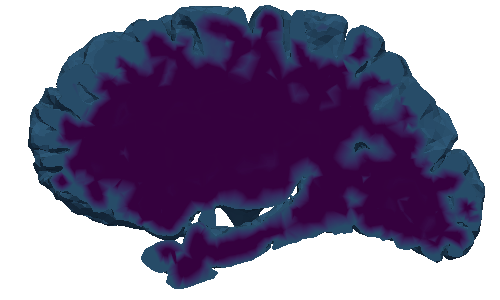
\includegraphics[width=0.4\textwidth]{./chapters/chp3/FIG/mri-tracer/2h}}&
    \imagetop{6h}&  \imagetop{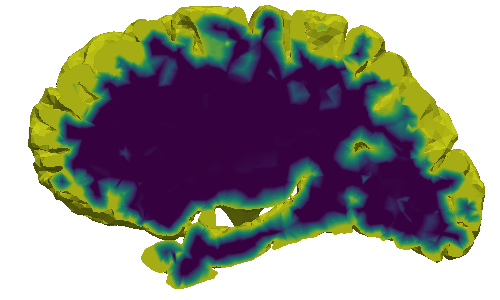
\includegraphics[width=0.4\textwidth]{./chapters/chp3/FIG/mri-tracer/6h}}\\
    \imagetop{12h}& \imagetop{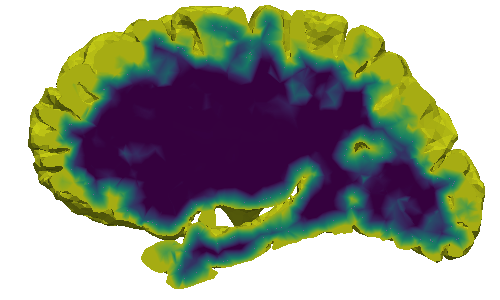
\includegraphics[width=0.4\textwidth]{./chapters/chp3/FIG/mri-tracer/12h}}&
    \imagetop{24h}& \imagetop{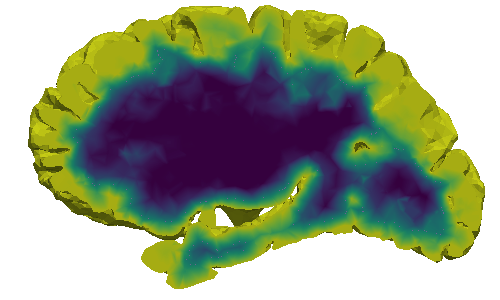
\includegraphics[width=0.4\textwidth]{./chapters/chp3/FIG/mri-tracer/24h}}\\
    \imagetop{48h}& \imagetop{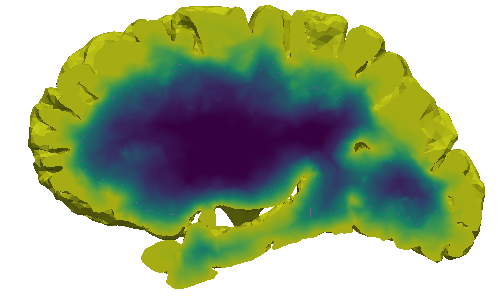
\includegraphics[width=0.4\textwidth]{./chapters/chp3/FIG/mri-tracer/48h}}&
    \imagetop{72h}& \imagetop{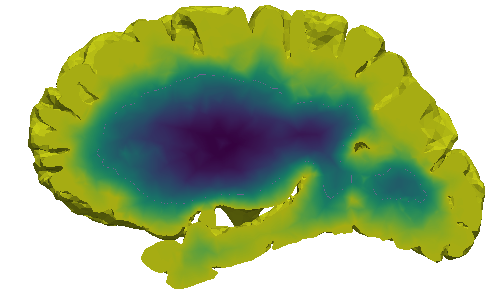
\includegraphics[width=0.4\textwidth]{./chapters/chp3/FIG/mri-tracer/72h}}
    \end{tabular}
    \caption{Simulated tracer concentration at given times (2, 6, 12,
      24, 48, 72h) post injection into subarachnoid CSF. Blue
      represents lower values, while yellow represents higher values.}
    \label{fig:chp3:approximate-numerical-soln}
\end{figure}


%% You can rotate the image by clicking in the viewing window
%% and while turning your mouse and holding the left mouse button down.
%% \begin{figure}\sidecaption
%% 	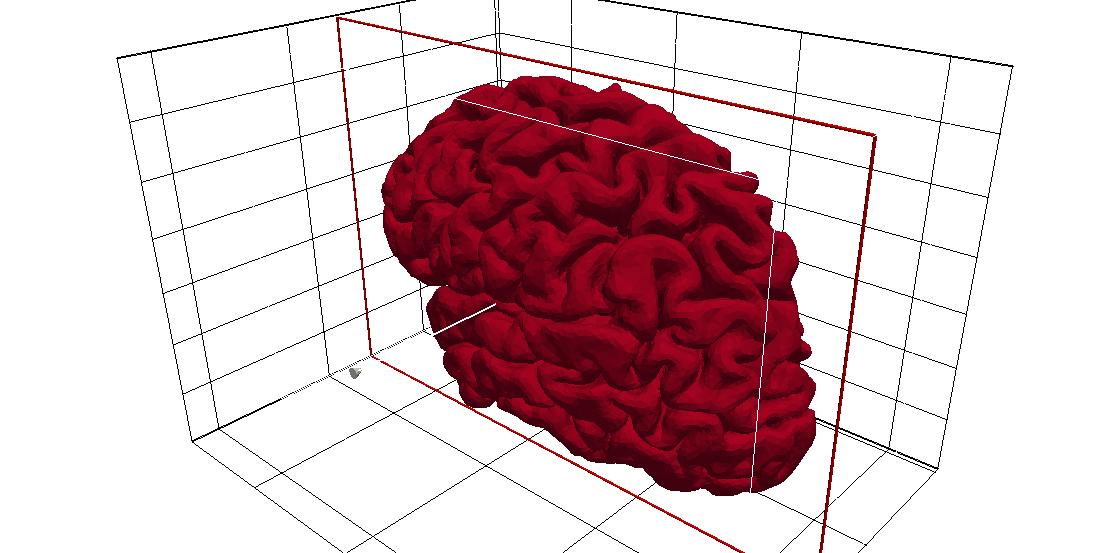
\includegraphics[width=0.630\textwidth]{./chapters/chp3/FIG/clip-plane}
%% 	\caption{The clip plane operation in ParaView}
%% 	\label{fig:chp3:paraview-clip}
%% \end{figure}
%% Since the tracer concentration was constant on the boundary you will notice that 
%% the entire left hemisphere is the same color. To see the variation in tracer 
%% concentration inside the brain we need to `clip' the mesh open. To do this click 
%% `Filters$\rightarrow$Alphabetical$\rightarrow$Clip ' in the menu bar.
%% You will see the 
%% left pane change to display the `Plane Parameters' that determine where the 
%% clip will occur.  You can modify these parameters if you wish and you will see
%% the red `clipping plane' change accordingly; c.f.~Figure \ref{fig:chp3:paraview-clip}.  
%% When you are satisfied with the location of the red clipping plane, click apply 
%% to slice the brain open for visualization of the tracer concentration within it.

%\begin{figure}
%    \begin{tabular}{l l l l}
%    \imagetop{30s}& \imagetop{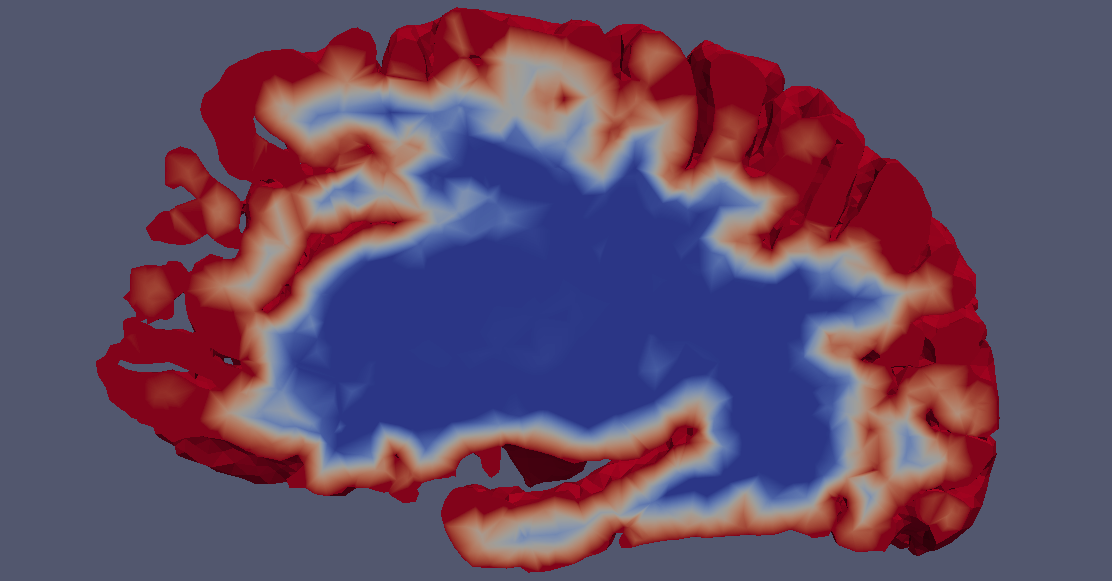
\includegraphics[width=0.49\textwidth]{./chapters/chp3/FIG/soltn-t30}} &
%    \imagetop{1m} & \imagetop{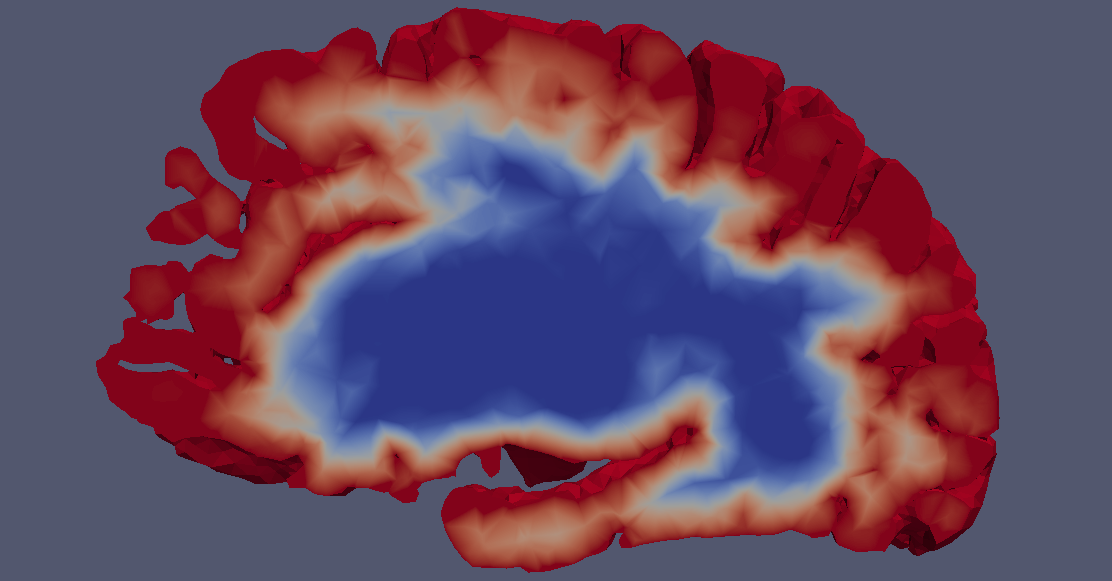
\includegraphics[width=0.49\textwidth]{./chapters/chp3/FIG/soltn-t60}}\\
%    \imagetop{2m} & \imagetop{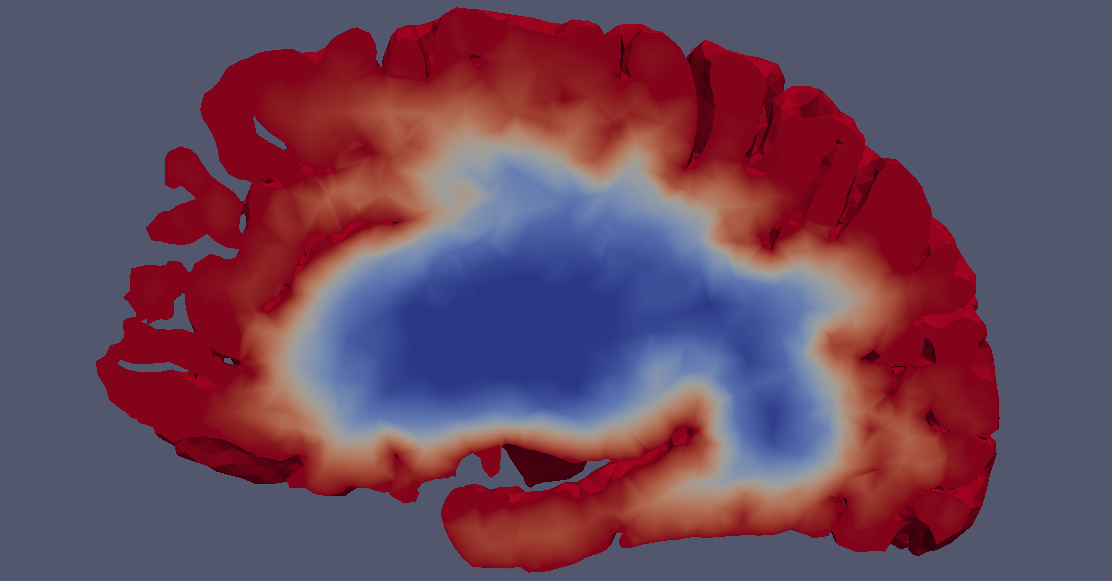
\includegraphics[width=0.49\textwidth]{./chapters/chp3/FIG/soltn-t120}} &
%    \imagetop{4m} & \imagetop{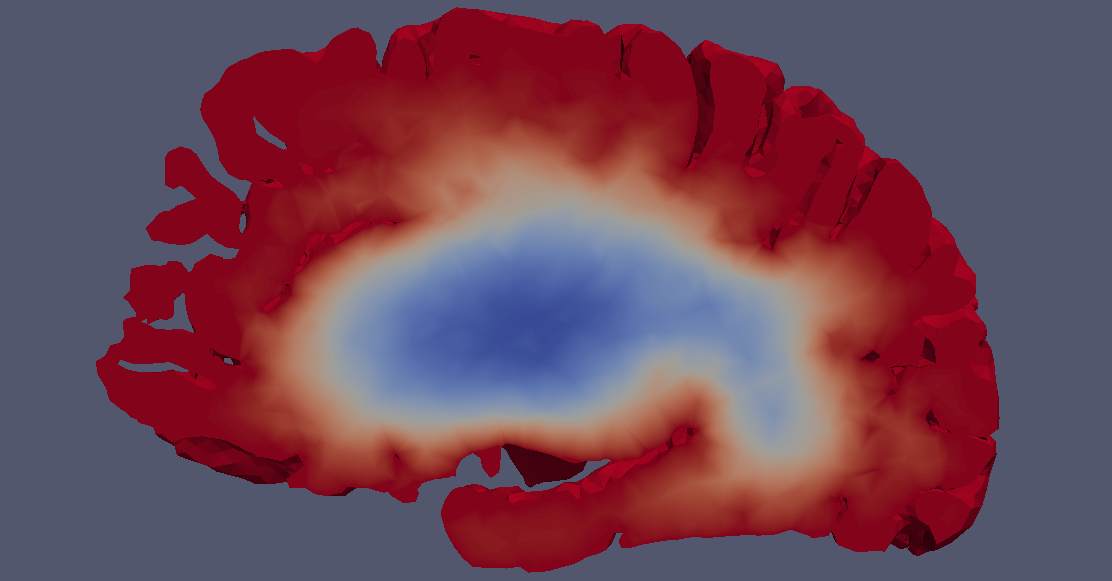
\includegraphics[width=0.49\textwidth]{./chapters/chp3/FIG/soltn-t240}}
%    \end{tabular}
%    \caption{Approximate distribution of tracer concentration (red is higher, %
%	blue is lower) at $t=30$ sec, $t=1$ min, $t=2$ min and $t=4$ min}
%    \label{fig:chp3:approximate-numerical-soln}
%\end{figure} 

%% After you have clipped your mesh you will want to rescale the displayed value,
%% which represents the concentration of the tracer, over all of the time steps
%% in the full series.  To do this, first select `solution.pvd', by clicking on
%% the name, in the top left pane.  Then, you will see options appear in the left
%% pane below the top-left window.  One of these options is titled `Coloring'.  
%% Moving and holding your mouse cursor over the buttons in this section will display
%% text telling you their functionality. Select the button that shows `Rescale to
%% data range over all timesteps'.  Clicking this button will start a process that
%% can take several minutes to complete.  After this completes you can view the 
%% result of the computation by clicking the green `play button' icon at the top
%% of the graphical interface just below the menu bar.  

%% If we modify the {\fenics} script \emp{chp3-diffusion.py} to print the 
%% concentration in the brain, $C_b$, at different time points we can evaluate the model
%% prediction for the concentration remaining in the subarachnoid CSF via 
%% $3.294\times 10^{-3} - C_b$.  We can then plot the percentage of tracer concentration
%% in the subarachnoid CSF relative to the initial concentration to visualize the uptake
%% of the tracer into the brain; this is plotted in figure \ref{fig:chp3:sas-tracer-perc}.

%% From figure \ref{fig:chp3:sas-tracer-perc} we can see that the model predicts that 
%% in 72 hours approximately 55\% of the gadobutrol tracer remains in the subarachnoid 
%% CSF so that 45\% has been diffusively absorbed by the brain tissue.  If we compare 
%% the images in figure \ref{fig:chp3:approximate-numerical-soln} to those of the actual 
%% tracer study for reference, or dementia, patients \cite{ringstand-2018-journal} we 
%% see that they do not match.  In particular, the tracer MRI intensity distributions of 
%% \cite{ringstand-2018-journal} show much more complex patterns than those of 
%% figure \ref{fig:chp3:approximate-numerical-soln}.  This is not bad news; it implies
%% that the brain is more complex than a simple sponge and that there is an exciting
%% modeling depth to be found in brain phenomena; even for simple clinical experiments.   



%% \subsection{SVM-Tk Implementation Details}
%% We implemented {\svmtk} for the purpose of constructing volume meshes using a closed surface. The process can be divided into two steps, the processing of the surface and the construction of the mesh. In general, surfaces can often have different types of defects, which need to be repaired so that the surface can be used for constructing meshes. %Furthermore, the construction of the mesh will require input parameters to ensure an appropriate computational volume mesh.

%% The idea of a volume mesh with subdomains defined by several overlapping and non-overlapping surfaces prompted the implementation of the \pythoninline{Surface} class. This means that each surface can be examined and repaired as needed, and subsequently used for constructing a mesh. The  \pythoninline{Surface} class was implemented with basic utilities, such as boolean operations, but also specific repair algorithms, like \pythoninline{isotropic\_remeshing}. We will go in more details about the implementation of core member functions, which includes functions that we have used earlier in this chapter.


%% %chosen set of concepts, where a concept is awell defined set of requirements
%% The core mesh construction process was implemented with the \pythoninline{Domain} class, which required the declaration of CGAL trait classes for domain and mesh. The domain class contains the information required to construct the mesh, while the mesh class contains the data structure of mesh, i.e. cells, facets and vertices, of the resulting mesh. %In CGAL, the domain classes have the copy constructor and assignment operator disabled, so we utilized unique pointer \kent{something missing in the explanation here. }to avoid the common pointer pitfalls in {\CC}. Furthermore, the disabled operations made iterative additions, such as push\_back and add, of surfaces impossible. 
%% The storing of the volume mesh as member variable was due to the limited number of implemented functions for the volume mesh, such as \pythoninline{save} and \pythoninline{remove\_subdomain}, and did not necessitate the implementation of a new class. However, if new functions are added, then the implementation of a Mesh class can be sought in the future. 

%% The structure of {\svmtk} included the CGAL headers when needed, and we declared the relevant CGAL trait classes with typedefs within each class. This implementation structure was used to avoid compilation errors due to hanging declarations while writing the code, and to avoid long variable names in the function implementation. We should note that the {\svmtk} is an active module, thus it can be subjected to additions, bug fixes and improvements, hence the implemented presented here may differ from the current implementation in the code repository. Additionally, not all functions are exposed to the python interface, and can therefore not be used with python.  

%% We will now go through some of the implementation of {\svmtk} in detail, focusing on the classes and functions that we have used. First, we have the code implementation of \pythoninline{Surface}. 
%% \begin{lstlisting}[style=CStyle]
%% class Surface
%% {
%% public:
%%   typedef CGAL::Exact_predicates_inexact_constructions_kernel Kernel; 
%%   typedef Kernel::Point_3 Point_3;   
%%   typedef CGAL::Surface_mesh<Point_3> Mesh;    
%%   typedef CGAL::Polyhedron_3<Kernel> Polyhedron;   
%%   typedef CGAL::Side_of_triangle_mesh<Mesh,Kernel> Inside; 

%%    // ----  Auxiliary ----
%%   typedef std::vector<Point_3>  Polyline_3; 
%%   typedef std::vector<Polyline_3> Polylines; 
%%   typedef std::vector<std::size_t>  Face;

%%     // --- Constructors ---
%%   Surface(){} 
%%   Surface(std::vector<Point_3>& points, std::vector<Face>& faces ); 
%%   Surface(const std::string  filename);

%%     // --- Boolean --- 
%%   void surface_intersection( CGALSurface& other);
%%   void surface_difference( CGALSurface& other);
%%   void surface_union( CGALSurface& other);    
    
%%     // --- Repair/Deformation  ---
%%   void isotropic_remeshing(double target_edge_length, unsigned int nb_iter, bool protect_border);
%%   void smooth_laplacian(const double c, int iter);
%%   void smooth_taubin(const size_t nb_iter);
%%   void separate_narrow_gaps();
%%   void collapse_edges();
%%   void collapse_edge(double target_edge_length);
%%   void fill_holes();
%%      .
%%      .
%%   void save(const std::string outpath);
%% protected:
%%   Mesh mesh;
%% }
%% \end{lstlisting}

%% %\kam{I have trouble with some of the names of the structures here. For instance, Kernel::FT FT. The name of the structure Kernel::FT should
%% %have a name that reflect or explain what it is. You can say the same about Tr etc. On the other hand for Kernel::Vector\_3, it is already
%% %stated that it is a 3\_vec. Why then include that in the name.  }
%% %\kam{mye traits. Forklare det? }
%% %\kam{hvorfor vises kun data-strukturer og ikke funksjoner? Du har jo mange spennende funksjoner som 
%% %surface\_intersection, union, collapse\_edges, fill\_holes, stitch\_borders, adjust\_boundaries, fair, insert\_point ..... }
%% First, we specified the CGAL kernel that we used for the implementation, which was the exact predicates inexact construction kernel. This kernel was determined to be best kernel in CGAL for the purpose of handling surfaces and constructing meshes. The kernel provides exact geometric predicates, i.e. inquiries about orientation, position and other methods that provide boolean or enum return values. However, the geometric construction may be inexact, due to round-off errors when constructing new points. The inexact kernel operations are subsequently faster than the exact construction kernels that also exists in CGAL, more details are found in \cite{schirra1998robustness}. 

%% We implemented the class with two different declarations of surface mesh, namely \emp{Polyhedron} and \emp{Mesh}. Both classes were used to handle triangulated surface mesh, but the \emp{Polyhedron} class used pointers and \emp{Mesh} used indices to structure the surface points. In most cases these meshes are interchangeable, and all functions in {\svmtk} are implemented to convert between the classes if needed. Therefore, we selected only the surface mesh was chosen as the class member variable.
%% \kent{Details missing.}\lmv{not much more to say, some function use polyhedron as input other use surface mesh. Most function handles both. }    

%% The class \pythoninline{Inside} was frequently used in the class functions to determine whether a point was inside another \pythoninline{Surface}. For instance, this function was used to evaluate if two surfaces overlap and needs to be separated. We have mentioned the function \pythoninline{separate\_narrow\_gaps} in Sec.~\ref{subsec:chp3:mesh-creation} has a method to avoid bridges in the cortical gray matter. This function has no arguments, as it will iteratively separate non-neighbor vertices until the distance between them was larger than the shortest connected edge.   
%% \kent{What is the convention? Classes start with upper case and functions start with lower case and use \_ for spacing? If so "Inside" is
%% not following the convention. } \lmv{ Inside is a typedef class}

 
%% The boolean operations listed in the header of \pythoninline{Surface} use functions implemented in CGAL\footnote{\url{https://doc.cgal.org/latest/Polygon\_mesh\_processing/index.html\#Coref\_section}}. These function may fail if the user specified a non-functional operation, like union of non-overlapping surfaces. We will use the union operation in Chapter~\ref{sec:chp4-left-right-tagged}, to create a union of the white matter surfaces.    

%% We used the function \pythoninline{isotropic\_remeshing} to reconstruct the loaded surface
%% so that each edge have similar length. The function has three arguments; the edge length, the number of iterations and protection of constrained edges. The function was implemented as a combination of two CGAL functions, \pythoninline{split\_edges} and \pythoninline{isotropic\_remeshing}. The function \pythoninline{isotropic\_remeshing} was implemented in CGAL using an incremental triangle-based isotropic remeshing algorithm. We decided to use the function \pythoninline{split\_edges} to handle the splitting of long protected constrained edges.%as CGAL recommended
%% This was due to the fact that if a protected edge was too long it can cause remeshing to fail by create an infinite loop of edge splits in the incident faces.    
 
%% We presented the function \pythoninline{smooth\_laplacian} in Chapter~\ref{fig:chp3:ernie-smoothing}. The implementation was based on the python module mshr,\footnote{\url{https://bitbucket.org/fenics-project/mshr/src/master/}}, which can be considered as a precursor to {\svmtk}. The function was implemented to determine the new position of a vertex by summation of all the connected edges as vectors. The resulting vector was then multiplied with a smoothing factor, the function argument.

%% The function \pythoninline{smooth\_taubin} was covered in Chapter~\ref{fig:chp3:ernie-smoothing} as a volume preserving smoothing algorithm. It was implemented by utilizing the  \pythoninline{smooth\_laplacian} with two different parameters $\mu$ and $\lambda$. These parameters are selected so that $0 < \mu < - \lambda$, further details are in \cite{taubin-1995-journal}. The arguments for taubin smoothing were set $\mu = 0.8$  and $\lambda=-0.805$. For other parameters, the user can use the \pythoninline{smooth\_laplacian} with specific parameters. \kent{Hasn't this already been said.  }\lmv{not directly but mentioned in ref{fig:chp3:ernie-smoothing}}

%% We have discussed the defects, such as holes, in Chapter~\ref{subsec:chp3:mesh-creation}. These defects can be corrected by FreeSurfer, but there can also be holes in the surfaces due to missing facets. The function \pythoninline{fill\_holes} followed the example provided in CGAL to add the missing facets. 

%% The overloaded function \pythoninline{collapse_edges} has two implementation. First, it can be used to collapse smaller edges than the provided input argument. Secondly, with no arguments, it can simplify structures by collapsing multiple edges in a straight line. For example, a structured cube surface with more than 8 vertices will be simplified to only have 8 vertices.

%% The \pythoninline{save} function was implemented to write the surface mesh to the file that was given as an argument. This can be used to inspect the processed surface, and determine if it can be used for mesh construction. Currently, we have two supported file formates, namely off and stl.

%% %The \pythoninline{svm.Domain} object is a combination of mesh domain and mesh in CGAL. 
%% The mesh construction used the concept of mesh domains, which represents the information required for the object to be discretized, that is boundaries, subdomains and  0-1 dimensions features. The \pythoninline{Domain} was implemented to automatically wrap the input surface to a function, this function was used to evaluate a point position relative to the surface, i.e., inside, outside or at the boundary. We will detail the main components of \pythoninline{Domain} header in the following code excerpt.
%% \begin{lstlisting}[style=CStyle]
%% class Domain{
%%  public :
%%    typedef CGAL::Exact_predicates_inexact_constructions_kernel Kernel;
%%    typedef Kernel::Point_3 Point_3;
%%    typedef CGAL::Mesh_polyhedron_3<Kernel>::type Polyhedron; 
        
%%    typedef CGAL::Polyhedral_mesh_domain_with_features_3<Kernel, Polyhedron> Polyhedral_mesh_domain_3; 
%%    typedef CGAL::Polyhedral_vector_to_labeled_function_wrapper<Polyhedral_mesh_domain_3, Kernel  > Function_wrapper; 

%%    typedef Function_wrapper::Function_vector Function_vector; 
%%    typedef CGAL::Labeled_mesh_domain_3<Kernel> Labeled_Mesh_Domain;
%%    typedef CGAL::Mesh_domain_with_polyline_features_3<Labeled_Mesh_Domain> Mesh_domain; 
%%    typedef CGAL::Sequential_tag Concurrency_tag;

%%    typedef CGAL::Mesh_triangulation_3<Mesh_domain,CGAL::Default,Concurrency_tag>::type Tr;

          
%%   template<typename Surface>        
%%   Domain(Surface& surface);
%%   template<typename Surface>     
%%   Domain(std::vector<Surface> surfaces);
%%   template<typename Surface>     
%%   Domain(std::vector<Surface> surfaces, 
%%          std::shared_ptr<AbstractMap> map);
        
%%   void remove_subdomain(std::vector<int> tags);
%%   void remove_subdomain(int tag);
%%   void save(std::string outpath);         
%%   void create_mesh(const double mesh_resolution );
%%   void create_mesh(double edge_size, double cell_size,
%%                    double facet_size, double facet_angle,
%%                    double facet_distance,
%%                    double cell_radius_edge_ratio);
%%  private :
%%   Function_vector v; 
%%   std::shared_ptr<AbstractMap> map_ptr;
%%   std::unique_ptr<Mesh_domain> domain_ptr;
%%   Minimum_sphere<Kernel> min_sphere; 
%%   C3t3 c3t3;
%%         ..    
%% }
%% \end{lstlisting}
%% %\kam{Many things here are not explained. Eg. C3t3. } \lmv{explained later on}
%% %\kam{Also, why typedefs within a class? }\lmv{ The reason behind typedefs in class, is twofold. First the experimental use of exact kernels, made it preferable to declare the template inside the classes, and in the future new implementation can benefit from this. The other reason was that making the typedefs global caused some conflicting declaration early on in the implementation, might not anymore, and therefore not chosen.}  
%% %\kam{I agree that it may be useful have typdefs within a class. However, it is not the most interesting thing about the
%% %class. The interesting thing, from a user-perspective, is what the class can do. It may also be interesting to know
%% %about the implementation, design choices etc. But then it should be explained. }
%% The class \pythoninline{Domain} starts by declaring the CGAL kernel and classes that was used in the implementation. The \pythoninline{Domain} class uses the exact predicates inexact construction kernel, which was covered for the case of \pythoninline{Surface}. 

%% The next batch of declarations concerns the wrapping of polyhedron surfaces to labeled mesh function, which allows for the construction meshes with indexed domains. First, we declared the triangulated surface structure with the class \emp{Mesh\_polyhedron\_3}, and used it together with kernel to define the mesh domain class for polyhedron \emp{Polyhedral\_mesh\_domain}. The labeled domain class was defined with \emp{Labeled\_Mesh\_Domain}, and the wrapping  of polyhedron to a labeled function with \emp{Function\_wrapper}. We declared \emp{Function\_vector}, so that multiple surfaces can be used to construct meshes.

%% The wrapping of surfaces to a labeled mesh domain was done, under the hood, in the constructor. This starts by creating a member variable vector of shared smart pointers to the object \emp{polyhedron\_domain} for each of the input surfaces. Then, the vector was used to declare the \emp{Function\_wrapper}, and subsequently used to create  unique smart pointer of the mesh domain object stored in the member variable \pythoninline{domain\_ptr}. 
%% We implemented \pythoninline{AbstractMap} as a virtual base class for the mapping of the different subdomain, which was created by overlapping surfaces. We will come back to this in Chapter~\ref{sec:chp4:tools:gray-white}, with the class \pythoninline{SubdomainMap}. 

%% The mesh construction required that we defined, the mesh domain, mesh criteria, the triangulation and the cell structure. We declared the volume mesh triangulation class with \emp{Mesh\_triangulation\_3}, and the cell structure with \emp{Mesh\_complex\_ 3}\emp{in\_ triangulation\_3}. The mesh was stored using the cell structure variable \pythoninline{c3t3}, which was also used for the triangulation. We would like to note an important distinction between the triangulation and the cell structure (mesh), as the triangulation can have vertices not connected to any cell in the mesh. The construction of isolated vertices can be minimized by sufficient preprocessing, but to ensure no isolated vertices, we implemented a function to remove all isolated vertices from the mesh.

%% We used the function \emp{create\_mesh} with the input of the \emp{mesh\_resolution} to determine the mesh criteria that was needed for CGAL. This was done with the struct \pythoninline{Minimum\_sphere}, which computes the minimum sphere radius needed to enclose all points in the polyhedron surfaces. We used the radius with the \emp{mesh\_resolution} input to set the maximum size of edges in the volume mesh. If the triangulated surfaces had smaller edges, then the smaller edges will be preserved in the constructed mesh. The function \emp{create\_mesh} also has the option to be initiated with the specific CGAL parameters; cell\_size, edge\_size , facet\_distance, facet\_angle and cell\_radius\_edge\_ratio. However, the user should have some familiarity with setting the CGAL parameters, since contradicting inputs may cause the mesh construction to crash.

%% The function \pythoninline{remove\_subdomain} was implemented to remove the subdomain from a constructed mesh. This requires that the user specifies a subdomain `tag', and it will remove all cells with the same `tag'. We can also remove multiple subdomains by adding the multiple `tags' to a vector and use the vector as the argument. This function and usage will be further detailed in Chapter~\ref{sec:chp4:tools:remove-vent:extraction}.

%% We can write the constructed mesh to file with the \pythoninline{save} function. This function will write the volume mesh to the provided file. There is currently only one supported file format, which is the medit file format. This file format is the default format for {\svmtk} and CGAL, and has the extension \emp{.mesh}.


\section{Advanced topics for working with larger cohorts}
\label{sec:chp3:advanced}

We have now covered the complete computational pipeline from MR images
to numerical simulation and visualization for a single imaging
modality, single stack of MRI data, and single simulation scenario. In
this section, we will cover some more advanced topics useful for
working with more complex DICOM data collections.

\subsection{Scripting the extraction of MRI series}

When processing larger DICOM datasets consisting of a large number of
patients and/or studies, the extraction of single MRI series via a
graphical interface can become tedious and error-prone. An alternative
approach is to script the extraction of specific MRI series using
FreeSurfer command-line utilities.

The extraction process consists of two command line steps: probing the
dataset for a given tag name and then extracting all data with the
given tag from the database. We will utilize the FreeSurfer command
\emp{mri\_probedicom} to examine and probe the DICOM metadata, so
ensure that FreeSurfer is installed and configured (see
Chapter~\ref{sec:chp2:tools:freesurfer}) before proceeding. The useful
command \emp{mri\_probedicom} can be used to compare the meta
data of different DICOM files with the flag \emp{-{}-compare} followed
by two DICOM filenames. We can also view the selected DICOM file by
using the flag \emp{-{}-view} e.g.:
\terminal{\$ cd \erniedicom/DICOM \\
\$ mri\_probedicom -{}-i IM\_0001 -{}-view
}
\noindent To probe the book DICOM data set for the tag "Protocol Name", which
associated with the numeric identifier 18 1030, issue the command
\terminal{\$ mri\_probedicom -{}-i IM\_0001 -{}-t 18 1030 \\
WIP T1\_3D
} 
\noindent The complete description of possible options to
\emp{mri\_probedicom} can be viewed by using the \emp{-{}-help} flag.

To extract files with a specific tag on the command-line, we can thus
probe each file, and copy files with a specific tag to a new
directory. This can be accomplished via e.g.~the following bash script
(also available at \emp{\coderoot/mri\_sort.sh}). The script
takes three types of input; the DICOM directory, the output directory and
an identifier for the protocol name.
\begin{lstlisting}[style=bashStyle]
#!/bin/bash
# 1st argument $1: input DICOM folder
# 2nd argument $2: the output copy directory
# 3rd argument $3: the identifier 

# Find all files in the directory and subdirectories
files=$(find $1 -type f ) 
for j in ${files}; do
    # Probe for protocol name (18 1030)
    name=$(mri_probedicom --i ${j} --t 18 1030) 

    # Check if identifier is part of protocol name.
    if [ "${name/$3}" != "$name" ]
       then
       # Copy file to (new) subdirectory 
       mkdir -p ${2}/${name//[[:blank:]]/}  
       cp ${j}  ${2}/${name//[[:blank:]]/} 
    fi
done
\end{lstlisting}

This script uses the bash command \emp{find} and the flag \emp{-type
  f} to find all files in the input directory and its
subdirectories. The script will go through all the files and probe
each file for the protocol name, and check if the protocol name
contains the identifier argument. Each file with the identifier in the
protocol name will be copied to a folder named by the protocol name in
the output directory. Spaces are removed from the protocol name --
this is preferred in order to avoid errors when using FreeSurfer.
Thus, we can use the script to extract all the images with \emp{T1}
string in the "Protocol Name" from the sample data set:
\terminal{\$ cd \erniedicom \\
\$ ./mri\_sort.sh ./DICOM ./ "T1" }

\subsection{More about FreeSurfer's recon-all}
\label{sec:chp3:advanced:recon-all}
The command \emp{recon-all} is the primary command for FreeSurfer,
since it will start the segmentation process. We have already
described the necessary flags for this command, but we will continue
the description with some additional options. This description will be
on an introductory level. However, the interested reader can use the
flag \emp{-help}, which will print detailed information about the
entire process and provide references to related articles and texts.

The command \emp{recon-all} is a sequential process that consist of 34
different stages, which are divided into three different
steps~\cite{freesurfer-wiki}. Data will be produced throughout the
process, and are often required as input for the next stage. We can
initiate each step separately by using the following flags instead of
\emp{-all}.
\begin{itemize}
\item \emp{-autorecon-1}: starts step-1 process that include stages 1-5, involving normalization and skull stripping. 
\item \emp{-autorecon-2}: starts step-2 process that include stages 6-23, involving the segmentation and surface generation.
\item \emp{-autorecon-2-pial}: starts construction of the surfaces that includes stages 16-23, involving various surface operations.  
\item \emp{-autorecon-3}: starts step-3 process that includes stages 24-34, involving 
statistical data generation and final parcellation.
\item \emp{-autorecon-all}: equivalent to \emp{-all} 
\end{itemize} 

These flags can be useful for restarting the segmentation. For
instance, if a failure occurred at stage 36, then we can start over
from stage 24 rather than from the beginning by using the flag
\emp{-autorecon-3}. This can also be useful, when it is necessary to
re-run the segmentation process after correcting an error. In
FreeSurfer there exist two types of errors, known as hard and soft
errors. Hard errors will terminate the segmentation process, while
soft errors are errors that we find in the produced data. The soft
errors are mostly segmentation errors, such as for example inclusion of the dura
in the segmentation and wrong segmentation of white matter. We can
edit the segmentation to correct the error, and run the recon-all with
the flag \emp{-autorecon-2-pial}. This will create new surfaces based
on the corrected segmentation files. The correction of soft errors
will not be further covered in this book; we rather refer to the
FreeSurfer documentation\cite{freesurfer-wiki}.

We continue with the flag \emp{-sd} that can be used to specify the
subject directory for the \emp{recon-all} command. This can be quite
useful in order to separate the segmentation data for different
cohorts. The segmentation of CSF filled structures, such as the
ventricular system, may require the additional use of T2-weighted MR
images to reach acceptable quality. We can include T2 MRI with the
flag \emp{-{}-T2}, and we can also use the flag \emp{-T2-pial} to use
the T2 MRI in the construction of the pial surfaces.

The segmentation in FreeSurfer is based on the segmentation atlas of
healthy subjects, therefore the segmentation can often encounter hard
errors for patients with abnormal brain anatomy. We can often allow
the segmentation to finish if we add the flag \emp{-notalairach},
which causes recon-all to skip assertion points in the first step. The
log of the recon-all script is documented in the folder \emp{scripts}
and all the specific command lines can be found in \emp{touch}.

%% We can also include multiple T1-weighted images to the command
%% process, this is done by reusing the input flag \emp{-i}. This is
%% mostly done for motion correction in MRI with motion artifacts.


